\section{Foreseen product specifications}%
\label{sec:org31f7574}
\subsection{QFD --- Quality Function Deployment}%
\label{sec:qfd}
The use of a QFD `Quality House' was opted as it is an efficient method of defining requirements laid out for the project and convert them into somewhat detailed engineering specifications in order to fullfill those requirements, along with several tools that allow to define the relations existing between the latter and the former.

The QFD works by using a matrix where the project requirements will be laid out as rows and the engineering specifications as columns; in the intersections lie a number representing the strength of the relationship requirement-specification.

Along with the requirements, the importance given to each is also specified, ranging from 1 (lowest importance) to 5 (highest importance) these, along with the number at each intersection, will be used to calculate the Weighted Score of each requirement and the Technical Importance Score of each specification. These results will in turn be used to calculate the importance of each specification and thus assign priorities for the Design Team.

Figure~\ref{fig:QFD} shows the `Quality House' for the RF CAR containing:
\begin{itemize}
\item Customer Requirements: Safe to Operate, Obstacle Avoidant, Fast, and so
  on.
\item Functional Requirements: Cost of Production, Maximum speed, Engine
  Power, amongst others.
\item The Intersection Values (referencing the strength of the
  requirement-specification correlation):
  \begin{itemize}
  \item 0: No Relation.
  \item 1: Weak Relation.
  \item 3: Moderate Relation.
  \item 9: Strong Relation.
  \end{itemize}
\item The Analytical Results, depicting, quantifiably, the relevance of each
  entity:
  \begin{itemize}
  \item Weighted Score, for the Requirements.
  \item Technical Importance Score, for the Specifications.
  \item Importance and Priority Rank, which are the main conclusion for which
    the QFD was used.
  \end{itemize}
\end{itemize}
For instance, the `engine power' specification and the `fast' requirement have a
very strong correlation (9) since the power of the engine is directly
responsible for the speed of the car.

With the QFD, the priorities ranks were obtained supplying the Design Team with a
straightfoward guideline. For instance, the cost of production should be
prioritized over all other specifications, followed by the maximum speed,
Ramp-Up Speed Time and so on.  On the other hand, the engine expectancy is of
little to no consequence (note that the importance added up to a mere 3\%),
followed by most of the camera-related specifications, this could be regarded as
a point of discussion, which should be prioritized? The functionality of the car
or the the feedback provided by the camera?

With the last point in mind, the QFD has the advantage of allowing further
discussion, simply by changing the importance of a requirement the priority ranking will change, ergo
the priorities can be altered, easily and efficiently, if deemed appropriate.
%
\begin{sidewaysfigure}[!htbp]
\centering
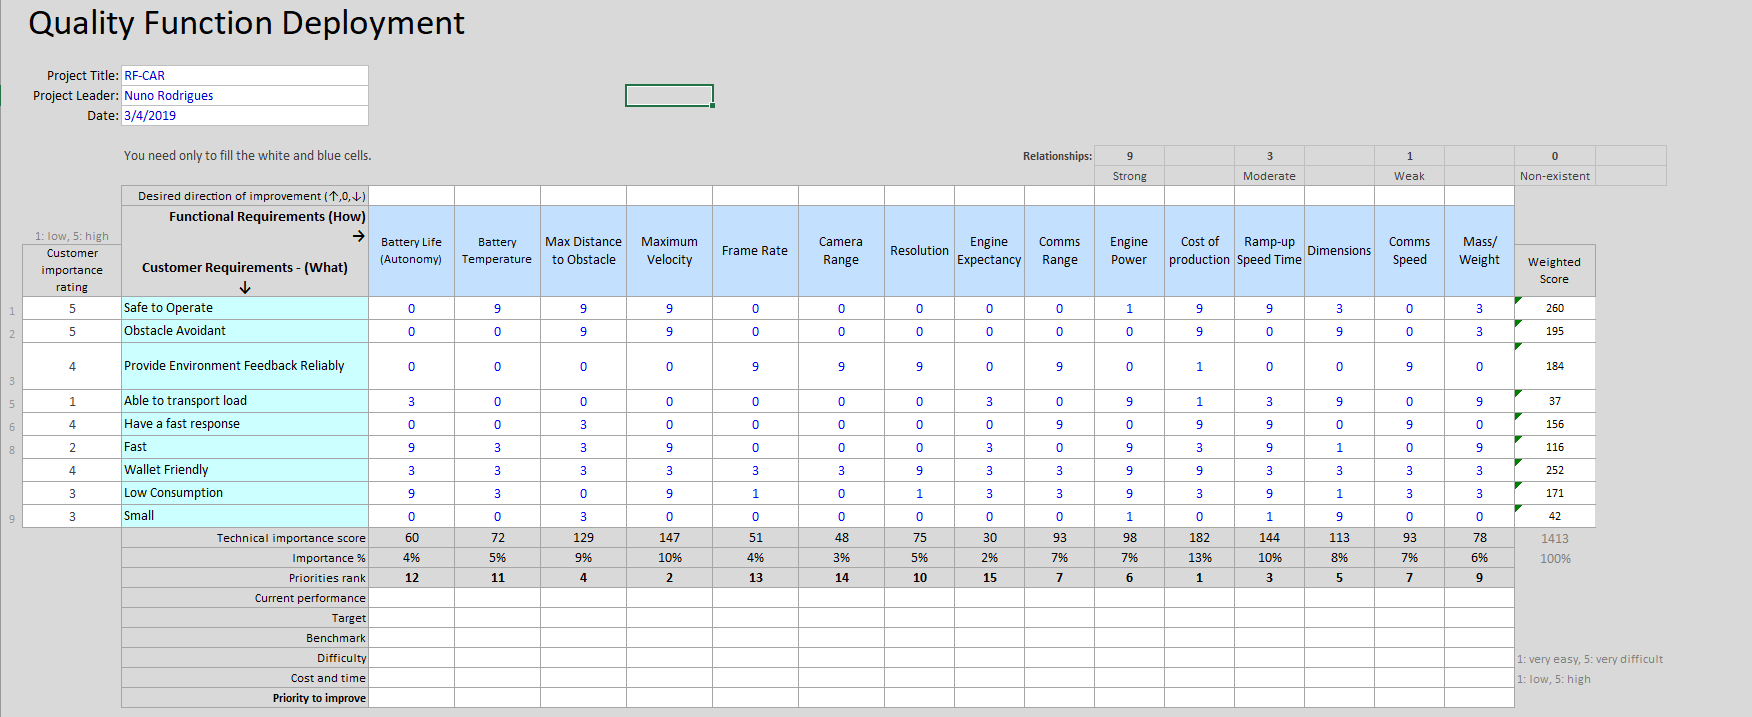
\includegraphics[width=1.25\textwidth]{./sec/img/QFD_Initial.png}
\caption{\label{fig:QFD}Foreseen product specifications:Quality Function Deployment for the RFCAR}
\end{sidewaysfigure}
\newpage
The foreseen product specifications are listed as topics below.

\subsection{Vehicle Autonomy}%
\label{sec:autonomy-specs}
The vehicle is operated in wireless mode, thus, a portable power source must be included. The autonomy referes to the time interval between battery fully charged and safely discharged and should be observed for the following scenarios:
\begin{itemize}
\item No load and vehicle operating at maximum speed;
\item No load and vehicle operating at mean speed;
\item Maximum load and vehicle operating at maximum speed;
\item maixmum load and vehicle operating at mean speed.
\end{itemize}
\subsection{Speed}%
\label{sec:speed-tests}
The vehicle must be operated within a safe range of speed, while also not increasing excessively the power consumption. Thus, these speed boundaries should be tested in the absence of an external load and in the presence of the maximum load.
\subsection{Safety}%
\label{sec:org83942c3}
Vehicle self integrity protection is a requirement in product design, especially considering the vehicle is to
be remotely operated. The safety of operation can be analysed in two ways, and considers the
preservation of people and goods. For the former, it is important to assure safe interaction as well as user operation --- the vehicle may encounter
several people along its path, but it must not inflict any damage. For the
latter, the vehicle under operating conditions must not inflict any damage to
goods. Thus, in the presence of conflicting user commands violating the safety
of people and goods, the local system should override them, taking corrective
measures to prevent it. The same holds true if the communication between user
and system is lost.
%The system uses odometric navigation.
%\item Human: Due to the odometric sensors safely fixed in the car, crashes will not occur, making it much harder for the car to hit a person or for any part of the car to jump and cause harm to the user or anyone around.
%\end{itemize}
\subsection{Image acquisition}%
\label{sec:image-acquisit}
The vehicle is equipped with a camera to assist in its navigation,
thus, requiring it to be fed to the user's platform appropriately.
\subsubsection{Frame rate}%
\label{sec:org5adf4ee}
Frame rate refers to the frequency at which independent still images appear on the screen. A better image quality is the result of a higher the frame rate but the processing overhead increases as well, so a compromise must be achieved between the quality of the image and the increaded processing overhead required. The minimum frame rate defined must be such that allows a clear view of the navigation.
\subsubsection{Range}%
\label{sec:orgecb044c}
How far can the camera capture images without loosing resolution and record them. The range must such that allows the user to see the obstacles when the car is heading to them and provide enough time to change the direction.
\subsubsection{Resolution}%
\label{sec:orgba87554}%
The amount of detail that the camera can capture. It is measured in pixels. The quality of the aquired image is proportional to the number os pixels but a greater resolution requires a greater data transfer and processing overhead, thus, a compromise must be achieved. The minimum resolution must be such that provides the least amount of information required for the user. 
\subsection{Communication}%
\label{sec:org4241610}
\subsubsection{Reliability}%
\label{sec:orgdcb920d}
A communication is reliable if it guarantees measures to deliver the data
conveyed in the communication link. As reliability imposes these measures, it
also increases memory footprint, which must be considered
depending on the case. For the devised product, an user command
must be acknowledged to be processed, otherwise, the user must be informed; on
the other hand, loosing frames from the video feed is not so critical — user can
still observe conveniently the field of vision if the frame rate is within
acceptable boundaries.
\subsubsection{Redundancy}
\label{sec:orgc5933fc}
The communication protocols are not flawless and the car relies on them to be controlled. If the communication is lost, the car cannot be controlled. A possible solution for this issue is using more communication protocols (e.g Wi-fi and bluetooth), so when one protocol fails, the car can still be controlled by the other.
\subsubsection{Range}%
\label{sec:org447a205}
The communication protocols have a limited range of operation, and, as such, regarding the environment on which the car is used the range can be changed.
The range refers to the maximum distance allowed between user and system for communication purposes.
\subsection{Responsiveness}%
\label{sec:org622e63a}
The movement of the car will be determined by the tilt movement of the smartphone. Sensibility refers to the responsiveness of the car on the minimum smartphone tilt movement. The sensibility must be in an range of values in which small unintentional movements will be enough to change the state of the car and it does not take big smartphone tilts for the car to move.
\subsection{Closed loop error}%
\label{sec:closed-loop-error-specs}
The speed, direction and safe distance to avoid colisions must be continuosly monitored to ensure proper vehicle operation. The closed loop error must then be checked mainly in three situations as a response to an user command:
\begin{itemize}
\item speed: the user issued an command with a given mean speed, which should be compared with the steady-state mean speed of the vehicle.
\item direction: the user issued an command with a given direction, which should be compared to the vehicle direction.
\item safe distance to avoid colisions: the user issued an command with a given direction and speed which can cause it to crash. The local control must influence, to prevent colision, and the final distance to the obstacles must be assessed and compared to the defined one.
\end{itemize}
\subsection{Summary}%
\label{sec:org1f95256}
Table~\ref{tab:specs-init} lists the foreseen product specifications.

% Please add the following required packages to your document preamble:
% \usepackage[table,xcdraw]{xcolor}
% If you use beamer only pass "xcolor=table" option, i.e. \documentclass[xcolor=table]{beamer}
% Please add the following required packages to your document preamble:
% \usepackage[table,xcdraw]{xcolor}
% If you use beamer only pass "xcolor=table" option, i.e. \documentclass[xcolor=table]{beamer}
\begin{table}[!hbt]
\centering
\caption{Specifications}%
\label{tab:specs-init}
%
\begin{tabular}{
>{\columncolor[HTML]{FFFFFF}}l 
>{\columncolor[HTML]{FFFFFF}}l 
>{\columncolor[HTML]{FFFFFF}}l }
\hline
                  & Values     & Explanation                                                                                                  \\ \hline
Autonomy          & 4 h        & \begin{tabular}[c]{@{}l@{}}Time interval between battery fully \\ charged and safely discharged\end{tabular} \\ \hline
Speed Range  & 0.1 to 1 m/s    & \begin{tabular}[c]{@{}l@{}}Speed at which the car can operate\end{tabular}              \\ \hline
Frame Rate        & 60 fps     & \begin{tabular}[c]{@{}l@{}}Frequency at which independent still \\ images appear on the screen\end{tabular}  \\ \hline
Camera Range      & 20 m       & \begin{tabular}[c]{@{}l@{}}How far can the camera capture images\\ without loosing resolution\end{tabular}   \\ \hline
Camera resolution & 480p       & Amount of detail that the camera can capture                                                                 \\ \hline
Comunication Range & 50 m & \begin{tabular}[c]{@{}l@{}}Maximum distance between the car and the\\ smarphone without losing connection\end{tabular} \\ \hline
speed Error    & 5 \%       & \begin{tabular}[c]{@{}l@{}}Maximum difference between desired \\ and real speed\end{tabular}              \\ \hline
Direction Error   & 5\%        & \begin{tabular}[c]{@{}l@{}}Maximum difference between desired\\  and real direction\end{tabular}             \\ \hline
Distance Error     & 5 \% & \begin{tabular}[c]{@{}l@{}}Maximum difference between desired\\ and real distance to the obstacle\end{tabular}         \\ \hline
Dimensions        & 20x12x5 cm & Dimensions of the car                                                                                        \\ \hline
Weight            & 0.5 kg     & Weight of the car                                                                                            \\ \hline
\end{tabular}
\end{table}

%%% Local Variables:
%%% mode: latex
%%% TeX-master: "../Phase1"
%%% End:
